% Fallback build of report.tex with the standard article class (use only if nle.cls is unavailable).
% Generated from report.tex: edit report.tex, not this file.
\documentclass[11pt,a4paper]{article}
\usepackage[margin=2.5cm]{geometry}
\usepackage[round]{natbib}
\makeatletter
\let\@origtitle\title \renewcommand\title[2][]{\@origtitle{#2}}
\let\@origauthor\author \renewcommand\author[2][]{\@origauthor{#2}}
\makeatother
\newcommand\ls{}\newcommand\ns{\ }\newcommand\received[1]{\date{#1}}
\newcommand\pagerange[1]{}\newcommand\pubyear[1]{}\newcommand\hpt{.}

\usepackage{graphicx}
\usepackage{url}
\def\UrlBreaks{\do\/\do\_\do\.}
\setlength{\emergencystretch}{2em}
\newcommand\TBD[1]{\textbf{[#1]}}
\newcommand\eg{{\it e.g.\ }}

\title[Detecting AI-Generated Text Across Domains and Generators]
      {Detecting AI-Generated Text Across Domains and Generators:\\
       Generalisation to Unseen Generators, Domains and Paraphrases}
\author[N.\ Kumar and others]
       {N\ls I\ls R\ls M\ls A\ls L\ns K\ls U\ls M\ls A\ls R,\ns
        V\ls I\ls V\ls E\ls K\ns K\ls U\ls M\ls A\ls R,\ns
        R\ls I\ls T\ls E\ls S\ls H\ns J\ls H\ls A\ns
        and\ns V\ls I\ls S\ls H\ls A\ls L\ns K\ls U\ls M\ls A\ls R\\
        Team 20, Deep Learning course, Sitare}

\received{22 November 2026}
\pagerange{\pageref{firstpage}--\pageref{lastpage}}
\pubyear{2026}

\begin{document}

\label{firstpage}
\maketitle

\begin{abstract}
Detectors of machine-generated text are usually evaluated on the same generators and domains they were trained on.
We study how well they generalise. Using the English part of the M4 benchmark (5 domains $\times$ 5 generators,
38,241 texts after cleaning), we compare a TF-IDF + logistic regression baseline, a fine-tuned RoBERTa classifier and
three zero-shot scores computed with GPT-2 medium (mean log-likelihood, log-rank and Fast-DetectGPT). Every detector is
evaluated in four settings: in-distribution, leave-one-generator-out, leave-one-domain-out, and a paraphrase attack
in which the same 500 machine texts are rewritten by a T5 paraphraser. Splits are made by group so that no human text,
or machine text written for the same prompt, appears in both training and test, and all methods are graded by one
shared evaluator (AUROC with group-bootstrap 95\% confidence intervals, accuracy and macro-F1 at a validation-chosen
threshold, and TPR at 1\% FPR). Fine-tuned RoBERTa and TF-IDF + LR are near-perfect in distribution (AUROC 0.991 and 0.990) and remain the strongest
detectors on unseen generators (mean 0.951 and 0.928), but the gap to zero-shot log-rank shrinks from 0.13 in
distribution to 0.02 on unseen domains. BLOOMZ is the hardest held-out generator for every detector. A T5 paraphrase
attack lowers the zero-shot scores by about 0.16 AUROC but barely affects the supervised detectors, which instead
flag paraphrased \emph{human} text as machine-written. We also find formatting artifacts in the M4 human texts that
supervised detectors exploit.
\end{abstract}

\section{Introduction}

Large language models (LLMs) now write fluent text in every domain, which creates a need to tell human-written text
from machine-generated text, for example in education and content moderation. Detectors fall into two families:
supervised classifiers trained on labelled examples, and zero-shot methods that score a text with a language model
without any training \citep{mitchell23}. A supervised detector can reach very high accuracy on the generators it was
trained on, but in practice a detector meets text from new generators, new domains, and text that was deliberately
rewritten to evade it.

The project brief (P20) asks us to distinguish human-written from LLM-generated text and to test generalisation to
unseen generators, using M4 \citep{wang24}, with a TF-IDF + LR baseline, a fine-tuned RoBERTa detector, zero-shot
perplexity / DetectGPT-style scoring and leave-one-generator-out evaluation, and to report cross-generator and
cross-domain robustness and the effect of paraphrasing attacks. Our contributions are:
\begin{itemize}
  \item a cleaned, group-aware version of M4 English with 12 evaluation settings (in-distribution, 5 held-out
        generators, 5 held-out domains, and a paraphrase before/after pair), released as split files;
  \item one shared evaluator so that every method is graded the same way, with guards against leakage;
  \item a comparison of five detectors across all settings, plus a length-only shortcut check;
  \item a paraphrase attack that keeps the human texts fixed, so the change in AUROC is caused by the paraphrase alone.
\end{itemize}

\section{Related work}

M4 \citep{wang24} is a multi-generator, multi-domain and multi-lingual benchmark for machine-generated text detection.
Its authors show that detectors trained on some generators or domains degrade on others, which motivates our
leave-one-out settings. DetectGPT \citep{mitchell23} observes that machine text tends to lie near a local maximum of
the model's log-probability and measures this \emph{probability curvature} by comparing the log-probability of a text
with that of perturbed copies. Fast-DetectGPT \citep{bao24} replaces the perturbations by an analytic estimate of the
same quantity computed from a single forward pass. Fine-tuned RoBERTa classifiers \citep{liu19} are a strong
supervised baseline for this task.

\section{Data}

\subsection{Source and sampling}
We use the English part of M4: human texts paired with texts generated for the same prompt by ChatGPT, davinci-003,
Cohere, Dolly-v2 and BLOOMZ, in Wikipedia, wikiHow, Reddit ELI5, arXiv abstracts and PeerRead reviews. The full
$5 \times 5$ grid exists; files that exist only for some domains (FLAN-T5, LLaMA) are left out so that every setting
covers the same generators. We keep at most 1,000 pairs per (domain, generator) cell (PeerRead: 250 papers per cell,
about four machine reviews each), drop texts under 50 characters and machine texts that copy the prompt, and use seed
42 throughout. The final dataset has 38,241 texts: 13,243 human and 24,998 machine, in 11,278 groups.

\subsection{Cleaning}
Three choices matter for a fair evaluation. (i) \emph{Whitespace is collapsed in every text}: arXiv and PeerRead human
texts contain hard line breaks that machine texts do not, which a detector could exploit as a formatting shortcut.
(ii) For BLOOMZ we take the output-only field, because its \texttt{machine\_text} field contains the prompt.
(iii) The same human text appears in up to five generator files; we keep it once and give it, and all its machine
twins, the same \emph{group} identifier (a hash of the human text; for PeerRead, of the paper).

\subsection{Evaluation settings and group-aware splits}
Splits are made by group, never by row, so no human text and no machine text written for the same prompt appears on
both sides of a split. Table~\ref{tab:settings} lists the settings.

\begin{table}
  \caption{Evaluation settings. All splits are by group. Sizes from \texttt{results/data\_audit.md}.}
  \resizebox{\textwidth}{!}{\begin{tabular}{llll}
  \hline\hline
  Setting & Train / val & Test & Question \\
  \hline
  \texttt{indist} & 80\% / 10\% of groups & other 10\% & same generators and domains \\
  \texttt{logo\_<gen>} ($\times$5) & other 4 generators & only \texttt{<gen>} & unseen generator \\
  \texttt{xdomain\_<dom>} ($\times$5) & other 4 domains & only \texttt{<dom>} & unseen domain \\
  \texttt{paraphrase\_orig} $\to$ \texttt{paraphrase} & \texttt{indist} model & 500 machine + 500 human & paraphrase attack \\
  \hline\hline
  \end{tabular}}
  \label{tab:settings}
\end{table}

\texttt{indist} has 30,602 / 3,801 / 3,838 texts; each LOGO test set has about 10,100 texts and each cross-domain
test set about 7,500. In a LOGO setting, the test groups keep only their human texts and the held-out generator's
texts; the other generators' texts in those groups are dropped rather than moved to training, so no test human text is
seen during training. Because each human text is kept once, machine texts outnumber human texts (about 1.9 : 1 in
\texttt{indist}); trained models use class weights, and AUROC does not depend on the ratio.

\section{Methods}\label{sec:methods}

Every detector outputs one score per text, with higher meaning more likely machine-generated.

\paragraph{Length-only baseline.} Logistic regression on log(characters) and log(words). It is not a real detector
but a shortcut check: where it scores well, part of every detector's score may come from text length.

\paragraph{TF-IDF + logistic regression.} Word 1--2-grams (up to 200k features) and character 3--5-grams (up to 300k
features) with sublinear TF, concatenated, then logistic regression with balanced class weights. The regularisation
strength $C \in \{0.25, 1, 4, 16\}$ is selected by validation AUROC in each setting.

\paragraph{Fine-tuned RoBERTa.} \texttt{roberta-base} with a two-class head, inputs truncated to 256 tokens, one epoch,
batch size 16, learning rate $2\cdot10^{-5}$ with AdamW, 6\% warm-up and linear decay, fp16 on a T4 GPU, and
class-weighted cross-entropy. Validation AUROC is computed twice per epoch and the best checkpoint is kept.

\paragraph{Zero-shot scores.} GPT-2 medium scores each text truncated to 256 tokens.
\emph{Log-likelihood} (\texttt{ppl}) is the mean token log-probability; \emph{log-rank} is minus the mean log-rank of
the actual tokens; \emph{Fast-DetectGPT} \citep{bao24} is
\[
  \frac{\sum_t \log p(x_t) - \sum_t \mu_t}{\sqrt{\sum_t \sigma_t^2}},
\]
where $\mu_t$ and $\sigma_t^2$ are the mean and variance of $\log p$ under the model's own next-token distribution at
position $t$. Because of the compute budget, Fast-DetectGPT scores a fixed subset of 1,500 texts (the 1,000
\texttt{paraphrase\_orig} test texts plus 500 balanced validation texts) together with the paraphrase test sets.

\paragraph{Paraphrase attack.} The 500 machine texts of the \texttt{paraphrase\_orig} test set are paraphrased sentence
by sentence with a T5 paraphraser (\texttt{humarin/chatgpt\_paraphraser\_on\_T5\_base}, nucleus sampling $p=0.9$,
temperature 0.8); sentences longer than 60 words are split first so the input is never truncated. The
\texttt{paraphrase} setting uses the same humans with the machine texts replaced, and every detector uses its
\texttt{indist} model without retraining. As a control, 200 human texts are paraphrased as well
(\texttt{paraphrase\_human}, label still human).

\section{Evaluation protocol}

All methods write predictions in one format and are graded by one script. True labels come from the dataset, never
from the detector, and the evaluator rejects any prediction file that scores a training text, misses a test text (only
Fast-DetectGPT may score a subset), or contains duplicate or non-finite scores. We report AUROC on the test set with a
95\% confidence interval from 1,000 bootstrap resamples of whole groups (texts in a group are not independent);
accuracy and macro-F1 at the threshold that maximises macro-F1 on the \emph{validation} set, applied unchanged to
test (omitted when validation has fewer than 50 texts per class); and the true positive rate at 1\% false positive
rate, reported only when the test set has at least 1,000 human texts.

\section{Results}

Tables~\ref{tab:indist}--\ref{tab:para} report test-set results; every number is read from the
\texttt{metrics.json} written by the shared evaluator (\texttt{results/tables.md}, generated by
\texttt{python -m src.make\_tables}). All 84 method--setting combinations (6 methods $\times$ 14 settings) were run. $^\dagger$Fast-DetectGPT is
scored on a subset (Section~\ref{sec:methods}), so its test sets are smaller (1,000 texts in distribution, 289--311 human and 150
machine texts per LOGO setting, 300 per cross-domain setting) and its intervals are wider; with fewer than 50
validation texts per class, its LOGO accuracy and F1 are not reported. Figure~\ref{fig:bars} summarises the
settings, Figure~\ref{fig:logo} shows the LOGO matrix and Figure~\ref{fig:para} the paraphrase attack.

\begin{table}
  \caption{In-distribution test results (\texttt{indist}).}
  \begin{tabular}{lcccc}
  \hline\hline
  Method & AUROC [95\% CI] & Accuracy & Macro-F1 & TPR@1\%FPR \\
  \hline
  Length only                & 0.591 [0.573, 0.610] & 0.651 & 0.589 & 0.004 \\
  TF-IDF + LR                & 0.990 [0.987, 0.992] & 0.952 & 0.947 & 0.836 \\
  Log-likelihood             & 0.845 [0.833, 0.856] & 0.777 & 0.758 & 0.229 \\
  Log-rank                   & 0.857 [0.846, 0.868] & 0.792 & 0.771 & 0.274 \\
  Fast-DetectGPT$^\dagger$   & 0.789 [0.761, 0.819] & 0.749 & 0.746 & -- \\
  RoBERTa                    & 0.991 [0.989, 0.993] & 0.954 & 0.949 & 0.868 \\
  \hline\hline
  \end{tabular}
  \label{tab:indist}
\end{table}

\begin{table}
  \caption{Leave-one-generator-out AUROC (column = held-out generator).}
  \begin{tabular}{lcccccc}
  \hline\hline
  Method & ChatGPT & davinci & Cohere & Dolly & BLOOMZ & Mean \\
  \hline
  Length only                & 0.478 & 0.580 & 0.585 & 0.504 & 0.764 & 0.582 \\
  TF-IDF + LR                & 0.995 & 0.962 & 0.963 & 0.904 & 0.814 & 0.928 \\
  Log-likelihood             & 0.964 & 0.823 & 0.956 & 0.816 & 0.744 & 0.860 \\
  Log-rank                   & 0.966 & 0.821 & 0.958 & 0.810 & 0.794 & 0.870 \\
  Fast-DetectGPT$^\dagger$   & 0.982 & 0.807 & 0.970 & 0.821 & 0.406 & 0.797 \\
  RoBERTa                    & 0.998 & 0.971 & 0.985 & 0.919 & 0.881 & 0.951 \\
  \hline\hline
  \end{tabular}
  \label{tab:logo}
\end{table}

\begin{table}
  \caption{Cross-domain AUROC (column = held-out domain).}
  \begin{tabular}{lcccccc}
  \hline\hline
  Method & Wikipedia & wikiHow & Reddit & arXiv & PeerRead & Mean \\
  \hline
  Length only                & 0.587 & 0.744 & 0.768 & 0.524 & 0.405 & 0.605 \\
  TF-IDF + LR                & 0.863 & 0.867 & 0.936 & 0.825 & 0.895 & 0.877 \\
  Log-likelihood             & 0.857 & 0.836 & 0.921 & 0.808 & 0.946 & 0.874 \\
  Log-rank                   & 0.877 & 0.841 & 0.938 & 0.814 & 0.955 & 0.885 \\
  Fast-DetectGPT$^\dagger$   & 0.868 & 0.682 & 0.814 & 0.799 & 0.826 & 0.798 \\
  RoBERTa                    & 0.845 & 0.844 & 0.983 & 0.907 & 0.935 & 0.903 \\
  \hline\hline
  \end{tabular}
  \label{tab:xdomain}
\end{table}

\begin{table}
  \caption{Paraphrase attack: AUROC on the same 500 machine and 500 human texts before and after paraphrasing.}
  \begin{tabular}{lcccc}
  \hline\hline
  Method & Original & Paraphrased & Drop & Human-paraphrase control \\
  \hline
  Length only                & 0.589 & 0.613 & -0.024 & 0.579 \\
  TF-IDF + LR                & 0.991 & 0.994 & -0.002 & 0.964 \\
  Log-likelihood             & 0.846 & 0.683 & 0.163 & 0.868 \\
  Log-rank                   & 0.860 & 0.699 & 0.160 & 0.880 \\
  Fast-DetectGPT$^\dagger$   & 0.789 & 0.743 & 0.046 & 0.789 \\
  RoBERTa                    & 0.990 & 0.984 & 0.006 & 0.970 \\
  \hline\hline
  \end{tabular}
  \label{tab:para}
\end{table}

\begin{figure}
  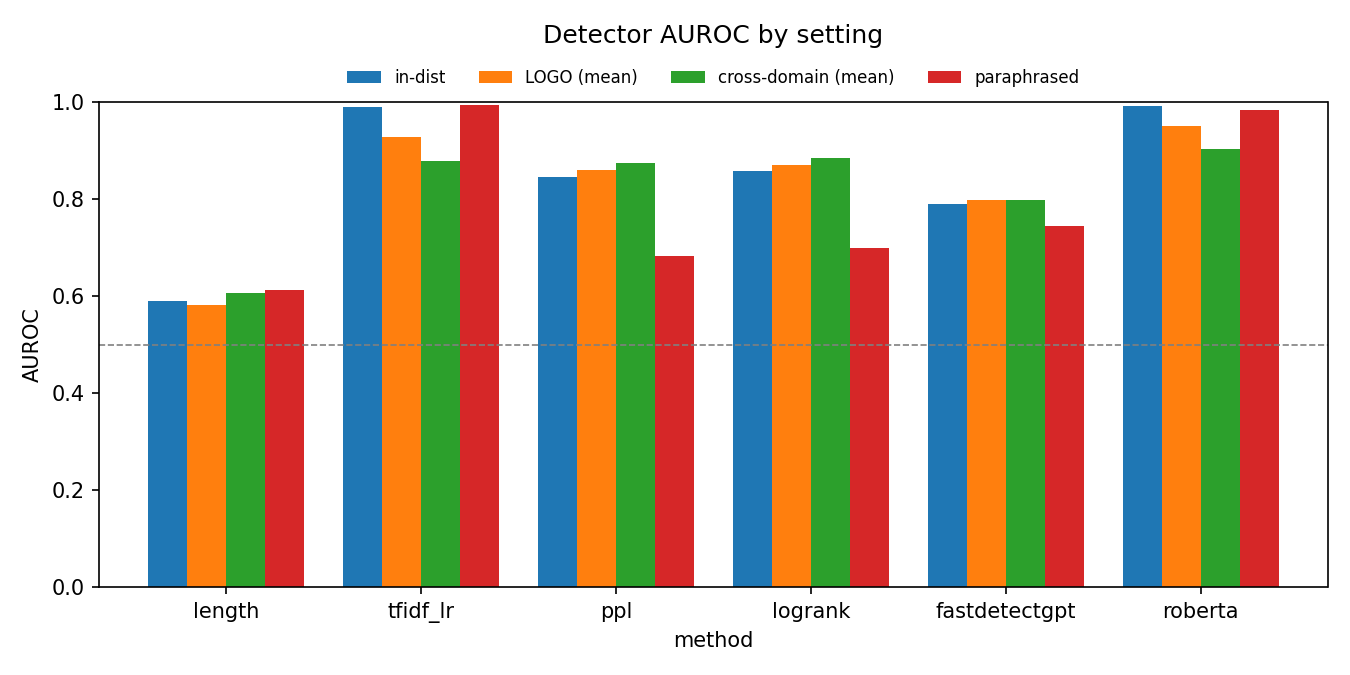
\includegraphics[width=\textwidth]{figures/fig1_auroc_by_setting.png}
  \caption{Test AUROC of each detector: in distribution, mean over the five held-out generators, mean over the five
  held-out domains, and after the paraphrase attack. Dashed line: chance.}
  \label{fig:bars}
\end{figure}
\begin{figure}
  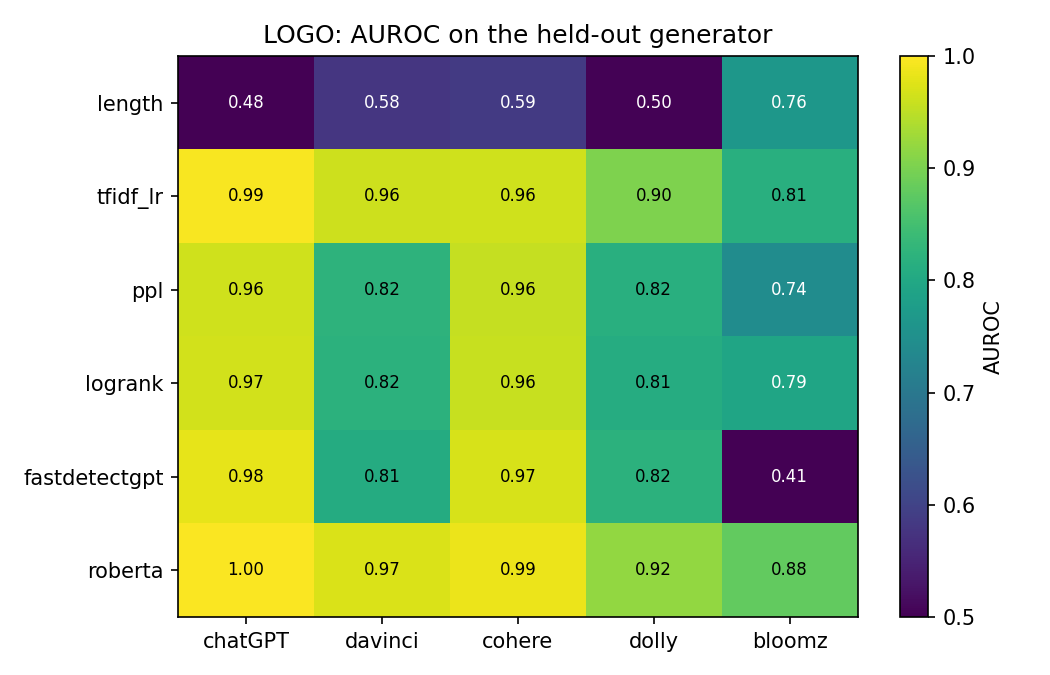
\includegraphics[width=0.8\textwidth]{figures/fig2_logo_heatmap.png}
  \caption{Leave-one-generator-out test AUROC (rows: detectors; columns: held-out generator).}
  \label{fig:logo}
\end{figure}
\begin{figure}
  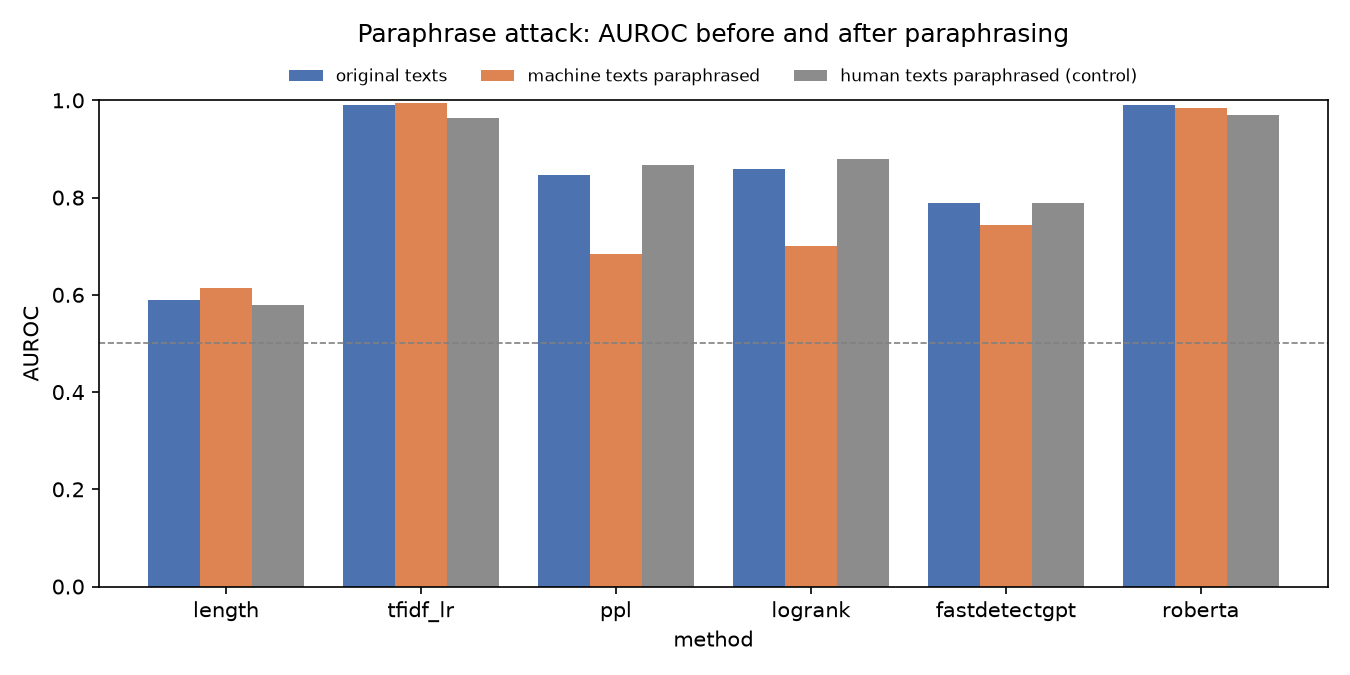
\includegraphics[width=\textwidth]{figures/fig3_paraphrase.png}
  \caption{Paraphrase attack (Table~\ref{tab:para}): test AUROC on the original texts, after paraphrasing the machine
  texts, and after paraphrasing 200 human texts instead (control). Dashed line: chance.}
  \label{fig:para}
\end{figure}

\section{Discussion}

\paragraph{Supervised detectors are strongest, but their advantage shrinks out of distribution.}
RoBERTa (0.991) and TF-IDF + LR (0.990) are almost perfect in distribution, and at 1\% FPR they still catch 87\% and
84\% of machine texts, against 23--27\% for the zero-shot scores. Both drop on unseen generators (means 0.951 and
0.928) and more on unseen domains (0.903 and 0.877). The zero-shot scores do not use training data, so their AUROC
stays roughly level across settings (log-rank: 0.857, 0.870, 0.885). As a result the gap between RoBERTa and
log-rank falls from 0.134 in distribution to 0.081 on unseen generators and 0.018 on unseen domains, and log-rank is
better than RoBERTa on held-out Wikipedia (0.877 vs 0.845) and PeerRead (0.955 vs 0.935).

\paragraph{BLOOMZ is the hardest unseen generator.} Every detector (not the length check) scores lowest when BLOOMZ is held out
(Table~\ref{tab:logo}); RoBERTa reaches 0.881 but only 23\% TPR at 1\% FPR. Fast-DetectGPT falls below chance there
(0.406): it ranks BLOOMZ texts as \emph{more} human than human texts. This rests on 150 machine texts and is not
shared by the other likelihood scores (log-likelihood 0.744, log-rank 0.794), so we report it as an observation;
we did not investigate the cause. ChatGPT is the easiest held-out generator for every detector (0.964--0.998); for the length check it is the reverse.

\paragraph{Length is a shortcut in some settings.} The length-only model is close to chance in distribution (0.591)
but reaches 0.764 with BLOOMZ held out and 0.768 and 0.744 on held-out Reddit and wikiHow, so in those settings
part of any detector's score may come from text length. On held-out PeerRead it is below chance (0.405): the
length relation learned on the other domains reverses there.

\paragraph{Paraphrasing defeats likelihood-based scores, not the supervised detectors.} On the same 500 machine
and 500 human texts, the attack lowers log-likelihood from 0.846 to 0.683 and log-rank from 0.860 to 0.699, and
Fast-DetectGPT less (0.789 to 0.743). RoBERTa loses only 0.006, and TF-IDF + LR none (0.991 to 0.994). The human
control explains why: when 200 human texts are paraphrased (label still human), the supervised detectors get
\emph{worse} (TF-IDF 0.991 to 0.964, RoBERTa 0.990 to 0.970), i.e.\ they score paraphrased human text as more
machine-like. They therefore react to the paraphraser's own style; the paraphraser used was itself trained on
ChatGPT outputs (\texttt{chatgpt\_paraphraser\_on\_T5\_base}), which may make its rewrites look machine-written to a
supervised model. The likelihood scores move the other way (log-rank control 0.880), consistent with paraphrasing
making any text less probable under GPT-2. The paraphrases changed the wording substantially (corpus BLEU 26.7
against the originals, no text unchanged) while keeping the length (ratio 0.97).

\paragraph{What the TF-IDF model uses.} The strongest machine features in distribution are words such as
\texttt{additionally}, \texttt{this article}, \texttt{examines} and \texttt{such as}. The strongest human features,
however, are formatting remnants (\texttt{references}, \texttt{external links}, \texttt{\_url\_0\_}, and the
pattern ``\texttt{. ,}'' left where wikiHow step titles were removed), which are not about who wrote the text. Section~\ref{sec:limits} discusses the
consequence.

\section{Limitations}\label{sec:limits}

\begin{itemize}
  \item We ran Fast-DetectGPT, the single-pass analytic form of DetectGPT's probability curvature, instead of
        perturbation DetectGPT \citep{mitchell23}, which needs about 20 T5 rewrites and 21 scoring passes per text and
        did not fit our GPU budget. Fast-DetectGPT scores a 1,500-text subset, so its LOGO and cross-domain
        estimates rest on fewer texts and have wider intervals.
  \item One zero-shot scorer (GPT-2 medium, 256 tokens); none of the M4 generators is GPT-2, so these methods are
        black-box here, and a stronger scorer could change their ranking.
  \item RoBERTa is trained for one epoch with default hyperparameters and a 256-token limit. Its validation set is
        used both for checkpoint selection and for the threshold, so its accuracy and F1 are slightly optimistic
        (AUROC is not affected).
  \item \emph{Formatting artifacts in M4 human texts.} The strongest ``human'' TF-IDF features in \texttt{indist}
        are leftovers of the source pages, not writing style: \texttt{references}, \texttt{external links}
        (Wikipedia section titles), \texttt{\_url\_0\_} (Reddit link placeholders) and the punctuation pattern
        ``\texttt{. ,}'' left where wikiHow step titles were removed (\path{results/tfidf_lr/indist/top_features.csv}).
        These leftovers are common in human texts and almost absent from machine texts: 51\% of human texts contain
        at least one of them against 2\% of machine texts (Wikipedia 97\% vs 4\%, wikiHow 99.8\% vs 3\%, Reddit 46\%
        vs 0.6\%; \texttt{results/artifacts.md}).
        Supervised detectors can partly exploit these, so their in-distribution scores are likely optimistic. We
        found this after the runs and did not have time to clean the data and rerun.
  \item For TF-IDF + LR, the selected $C$ was the largest value in the grid ($C=16$) in every setting, so a larger
        $C$ might be slightly better; validation gains between $C=4$ and $C=16$ were about 0.001 AUROC.
  \item English only, at most 1,000 machine texts per cell, one paraphraser, and one seed: the confidence
        intervals capture test-set sampling, not training variance.
\end{itemize}

\section{Conclusion}

On M4 English, fine-tuned RoBERTa is the most accurate detector in every setting, but its lead over a zero-shot
log-rank score nearly vanishes on unseen domains, and BLOOMZ remains hard for every detector when it is not seen in
training. A sentence-level paraphrase attack mainly hurts likelihood-based detectors, while supervised detectors
appear robust partly because they flag the paraphraser's style rather than machine authorship. Formatting artifacts
in the human texts mean that in-distribution scores of supervised detectors on M4 should be read as optimistic.

\section*{Reproducibility}
All code, split files and results are in the team repository
(\url{github.com/NIRMAL20062/generated_text_detection}). Every run writes \texttt{run\_info.json} with the git
commit, seed, hyperparameters, hardware and runtime; the README lists every command, and each script has a
\texttt{--dev} mode that runs on a committed sample in under two minutes.

\section*{Author contributions}
N.\ Kumar: data pipeline, splits, shared evaluator, baselines, tables. Vivek Kumar: RoBERTa detector.
R.\ Jha: zero-shot detectors, RoBERTa training script and Kaggle notebook, paraphrase attack script.
Vishal Kumar: paraphrase attack results, results tables and figures, error analysis, formatting-artifact analysis, report assembly.

\begin{thebibliography}{}
  \bibitem[Bao {\it et al.}(2024)]{bao24}
   Bao, G., Zhao, Y., Teng, Z., Yang, L. and Zhang, Y. (2024) Fast-DetectGPT: efficient zero-shot detection of
   machine-generated text via conditional probability curvature. In {\it International Conference on Learning
   Representations (ICLR)}. arXiv:2310.05130.
  \bibitem[Liu {\it et al.}(2019)]{liu19}
   Liu, Y., Ott, M., Goyal, N., Du, J., Joshi, M., Chen, D., Levy, O., Lewis, M., Zettlemoyer, L. and Stoyanov, V.
   (2019) RoBERTa: a robustly optimized BERT pretraining approach. arXiv:1907.11692.
  \bibitem[Mitchell {\it et al.}(2023)]{mitchell23}
   Mitchell, E., Lee, Y., Khazatsky, A., Manning, C. D. and Finn, C. (2023) DetectGPT: zero-shot machine-generated
   text detection using probability curvature. In {\it International Conference on Machine Learning (ICML)}.
   arXiv:2301.11305.
  \bibitem[Wang {\it et al.}(2024)]{wang24}
   Wang, Y., Mansurov, J., Ivanov, P., Su, J., Shelmanov, A., Tsvigun, A., Whitehouse, C., Mohammed Afzal, O.,
   Mahmoud, T., Sasaki, T., Arnold, T., Aji, A. F., Habash, N., Gurevych, I. and Nakov, P. (2024) M4:
   multi-generator, multi-domain, and multi-lingual black-box machine-generated text detection. In {\it Proceedings
   of EACL}. arXiv:2305.14902.
\end{thebibliography}

\label{lastpage}

\end{document}
